\documentclass[i3]{oss}
\usepackage[english]{babel}
\usepackage{graphicx}

\usepackage{fullpage}
\usepackage{color}
\usepackage{soul}
%\usepackage{gensymb}
\usepackage{caption}
\usepackage{subcaption}
\usepackage[section]{placeins}
\usepackage{titlesec}
\usepackage{wrapfig}
\usepackage{color}
% Automatically introduces paragraph spacing
\usepackage{parskip}

% Lets Latex correctly interpret the symbols: < >
\usepackage[T1]{fontenc}

\setcounter{secnumdepth}{4}
\titleformat{\paragraph}
{\normalfont\normalsize\bfseries}{\theparagraph}{1em}{}
\titlespacing*{\paragraph}
{0pt}{3.25ex plus 1ex minus .2ex}{1.5ex plus .2ex}

\newcommand{\class}[1]{\texttt{#1}}
\newcommand{\method}[1]{\texttt{#1}}
\newcommand{\junit}{\emph{JUnit }}
\newcommand{\Daemon}{\class{Daemon  }}
\newcommand{\gloss}[1]{\textbf{#1}}
\newcommand{\col}[1]{\textcolor{red}{#1}}
\newcommand{\comment}[1]{{\huge \textcolor{green}{#1}}\\}

\begin{document}

\members{Joren Verspeurt {\small \texttt{(r0258417)} } \\ %# Commentaar
         Sophie Marien {\small \texttt{(s0216517)}}\\
         Stef Noten {\small \texttt{(s0211264)}}\\
         Toon Nolten {\small \texttt{(r0258654)}} \\
         Begeleider: Mario H. C. T.} % teamleden

\maketitlepage
\newpage
\tableofcontents
\pagebreak




%-----------------------------------------------------------------------
%	INLEIDING
%-----------------------------------------------------------------------
\section*{Introduction}
\label{ssec:introduction}
%introductie en de belangrijkste elementen van ons ontwerp
In the first iteration we assessed the design and implementation of \junit and in the second iteration we had to extend it with a daemon that would continuously test a given project according to a policy chosen by the user.
In this iteration we have to expand \junit to combine multiple policies. The combining of policies have to be done in a fair way.

In section \ref{ss:designext} and \ref{ss:implemenext} we discuss the implementation of the composition of the policies and the design of this extension is explained.
In section \ref{ss:refactoring} and \ref{ss:analyse} the refactoring and the analyses of our extension of \junit are discussed. 
At the end we discuss the project and give an evaluation.

\section{Activity 1}
\subsection{Design}
\label{ss:designext}

The Composite pattern is used to support composing different \class{Policy}s in a fair way.
This fairness, according to the assignment, is the kind of fairness such as in the context of process scheduling.
In our case this means that the child \class{Policy}s of a composite \class{Policy} can all choose in turns which test should be next in the order.  

\subsection{Implementation of the extension}
\label{ss:implemenext}

For the third iteration the functionality of the policies will be extended. 
It should be possible to combine multiple sorting policies.
The order imposed by a combined policy is derived by allowing each policy to determine the next test in a turn based fashion.\\

In our implementation all of the policies will determine an order for the tests to be run. All these lists with test that have an order provided by the policy will be merged with each other. The merging will be as follow: 
\begin{itemize}
\item First it will take one Policy and take the first test in the list and put this test as first.
\item Second it will look in the other lists of tests of the other policies if this test is in the list. If this test is an element of the list it will be discarded. 
\item Third the second Policy will say which test it will be given.
\item Again we will check in the other lists if this test is in the list.
\item This will go on until no tests are left in the lists.
\end{itemize}

Instead of that we will see what the order is of the tests we will ask the Policies which order they want to give to the test. We will do this because if a Policy has no data for a test it can not give an order to this test. If it cannot give an order to a test it is no use to let this policy decide when this test will be set. 


\begin{table}[h!]
\begin{center}
    \begin{tabular}{ c  c  c  c | c}
     \class{Policy 1} & \class{Policy 2} & \class{Policy 3} & \class{Policy 4} & Order  \\ \hline
    	A & B & A & E & A \\
        B & D & B & D & B \\
        C & E & C & G & C\\
        D & G & F & \col{I'} & E \\
        E & F & J & \col{H'} & D \\
        F & \col{A'} & \col{G'} & \col{B'} & G \\
        G & \col{C'} & \col{H'} & \col{A'} & F \\
        H & \col{I'} & \col{D'} & \col{J'} & J \\
        \col{I'} & \col{J'} & \col{E'} & \col{C'} & H \\
        \col{J'} & \col{H'} & \col{J'} & \col{F'} & \col{I'} \\
    \end{tabular}
    \caption{Example of the merging of policies }
    \label{fig:orderex}
    \end{center}
\end{table}

Figure \ref{fig:orderex} gives an example of the merging of the policies. The test are A to I. If a policy has no data about a test and can thus not give an order to the test it is marked with an accent ('). When the resulting order of test is made, it will not take into account the tests with an accent. It will proceed with the following policy. If all policies have only tests with no order left the merging will stop and the tests with an accent will be put at the end of the list.

 

\section{Activity 2}

Activity 2 consists of the refactoring of our code from iteration 2 and the analysis of the final code with the refactoring. 

\subsection{Refactoring}
\label{ss:refactoring}
There are two mayor refactorings done. One in the \Daemon and one in the \class{ConsoleView}. \Daemon is responsible for repeatedly running a collection of tests as well as creating everything needed by policies.
This includes a \class{RunNotifier} which notifies listeners of events while running tests. A data enroller and a statistic provider also is created.

The \Daemon was implemented as a facade but it contains too much functionality.
For example testruns are now handled manually by \Daemon, but this is
not a responsibility of \Daemon, a possible solution is to add a class
that represents testruns.

The \class{ConsoleView} adds a way to handle interaction with the user. 
When the \class{ConsoleView} starts, the user is asked for the desired policy.
It subscribes itself on the \class{Daemon} and starts it. For the events it receives, it outputs a textual representation. 
Additionally, a menu is implemented: a user can always press the \emph{<ENTER>} key, to view a list of options. Implemented options include changing the policy, queueing a new testrun and stopping the program. \\


In the previous iteration the \Daemon class had too many responsibilities. 
This was refactored and the responsibilities of \Daemon were divided over three different classes: \class{Launcher}, \class{TestRun} and \class{TestRunCreator}.

The responsibility for creating the necessary objects and doing the necessary configuration for starting the \Daemon was placed in \class{Launcher}. 
The \class{Launcher} acts like a facade to our extension as it provides a simplified interface to its functionality.

The responsibility for running tests was abstracted into \class{TestRun}.
\class{TestRun}s can be created according to a specific \class{Policy} by using the \class{TestRunCreator}. \class{TestRun}s can also be created without a specific \class{Policy} by using the \class{TestRunCreator}.
Doing the instantiation in this way decouples \class{TestRun} from \class{Policy} in a way that maintains its generality. 

Another refactoring was done in the class \class{ConsoleView}. The responsibility of the menu of the consoleview is now placed in the \class{MenuAction}. 






\subsection{Analysis}
\label{ss:analyse}


%-----------------------------------------------------------------------
%	PROJECT MANAGMENT
%-----------------------------------------------------------------------
\section{Project management}
\label{ssec:Projectmanag}
%Een beschrijving van de taakverdeling voor elk teamlid: een concrete beschrijving van
%elke taak en activiteit en de tijd die hierin werd genvesteerd.
% Een schatting van de totale tijd die elk teamlid in dit project heeft genvesteerd

The division of tasks was about the same for everybody. Because it was a small task the design and the implementation was done together. In table \ref{tab:werkuren} the workhours per teammember can be seen for the different parts of the assignment. The different parts are various (setting up eclipse, visual paradigm, \junit, .. ), design, implementation and report. 

We had a lot discussion about the fairness of the ordening of the tests by a composite of policies. The assignment was not very clear and there were two different oppinions about it.  



%TODO tekst


\begin{table}[h!]
\begin{center}
    \begin{tabular}{ r | c  c  c  c  c  c}
     & Joren & Toon & Stef & Sophie \\ \hline
    	Various & 		3u30 & 4u00 & 4u00 & 4u00\\
        Design & 		14u30 & 20u30 & 25u00 & 20u30 \\
        Implementation & 28u00 & 34u30 & 40u30 & 16u50\\
        Report & 		18u00 & 16u00 & 21u00 & 16u40 \\
        Total & 		00u00 & 00u00 & 00u30 & 00u00  
    \end{tabular}
    \caption{Overview of the workhours per subject}
    \label{tab:werkuren}
\end{center}
\end{table}

%TODO figuren updaten
\begin{figure}[h!]
        \centering
        \begin{subfigure}[hb]{0.20\textwidth}
                \centering
                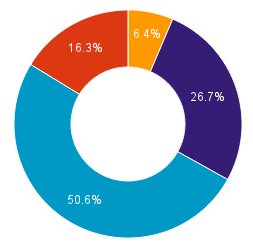
\includegraphics[width=\textwidth]{chart_2}
                \caption{Joren}
        \end{subfigure}%
        \begin{subfigure}[hb]{0.20\textwidth}
                \centering
                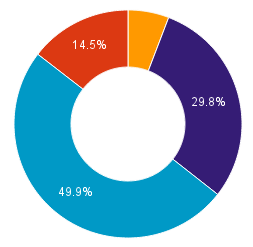
\includegraphics[width=\textwidth]{chart_3}
                \caption{Toon}
        \end{subfigure}%
        \begin{subfigure}[hb]{0.20\textwidth}
                \centering
                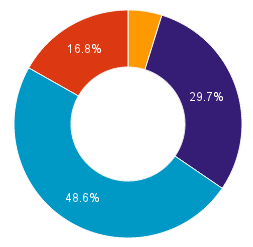
\includegraphics[width=\textwidth]{chart_4}
                \caption{Stef}
        \end{subfigure}%
        \begin{subfigure}[hb]{0.20\textwidth}
                \centering
                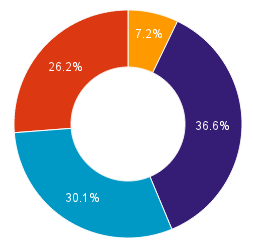
\includegraphics[width=\textwidth]{chart_5}
                \caption{Sophie}
        \end{subfigure}%
                \begin{subfigure}[hb]{0.20\textwidth}
                \centering
                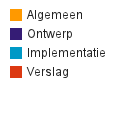
\includegraphics[width=\textwidth]{legende}
                \caption{Legend}
        \end{subfigure}%


 \caption{Overview of the division of tasks}
\label{fig:werkverdeling}
\end{figure}

\section{Glossary}
\label{ssec:glossary}
\begin{description}

\item \gloss{item}
ekjrelkrj

\end{description}
 

\end{document}